% Created by tikzDevice version 0.12.6 on 2024-10-30 10:02:59
% !TEX encoding = UTF-8 Unicode
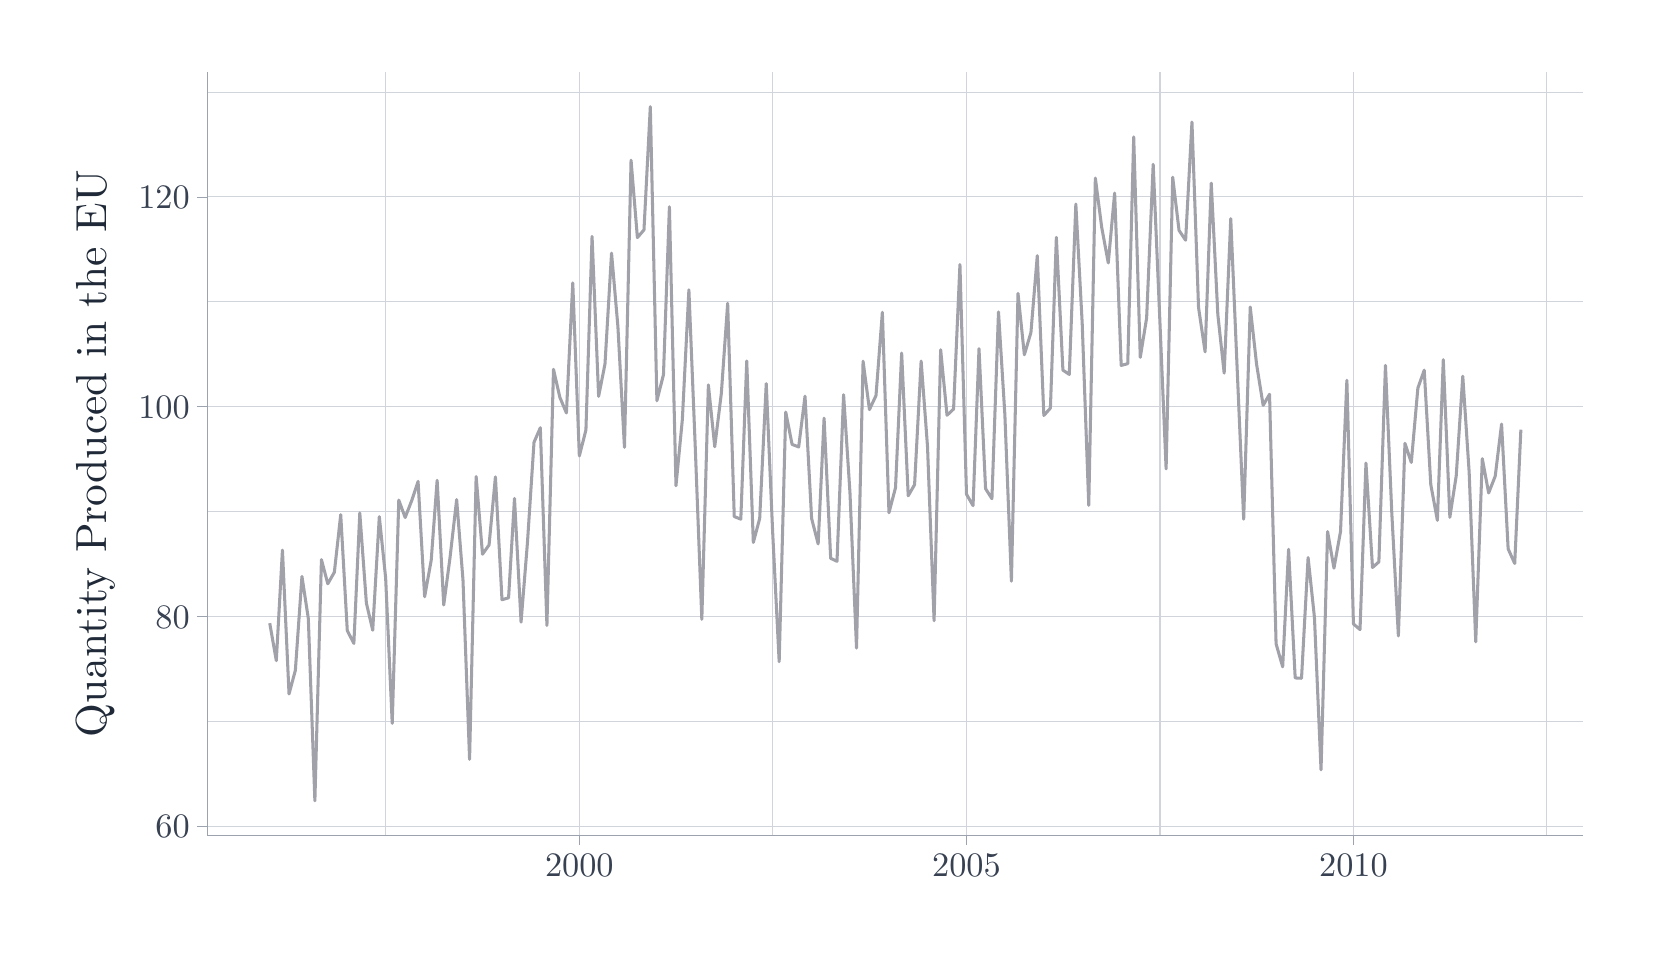
\begin{tikzpicture}[x=1pt,y=1pt]
\definecolor{fillColor}{RGB}{255,255,255}
\path[use as bounding box,fill=fillColor] (0,0) rectangle (578.16,325.21);
\begin{scope}
\path[clip] (  0.00,  0.00) rectangle (578.16,325.21);
\definecolor{drawColor}{RGB}{255,255,255}

\path[draw=drawColor,line width= 0.7pt,line join=round,line cap=round,fill=fillColor] (  0.00,  0.00) rectangle (578.16,325.21);
\end{scope}
\begin{scope}
\path[clip] ( 64.86, 33.29) rectangle (562.16,309.21);
\definecolor{drawColor}{RGB}{255,255,255}
\definecolor{fillColor}{RGB}{255,255,255}

\path[draw=drawColor,line width= 0.7pt,line join=round,line cap=round,fill=fillColor] ( 64.86, 33.29) rectangle (562.16,309.22);
\definecolor{drawColor}{RGB}{209,213,219}

\path[draw=drawColor,line width= 0.4pt,line join=round] ( 64.86, 74.59) --
	(562.16, 74.59);

\path[draw=drawColor,line width= 0.4pt,line join=round] ( 64.86,150.37) --
	(562.16,150.37);

\path[draw=drawColor,line width= 0.4pt,line join=round] ( 64.86,226.16) --
	(562.16,226.16);

\path[draw=drawColor,line width= 0.4pt,line join=round] ( 64.86,301.94) --
	(562.16,301.94);

\path[draw=drawColor,line width= 0.4pt,line join=round] (129.43, 33.29) --
	(129.43,309.21);

\path[draw=drawColor,line width= 0.4pt,line join=round] (269.29, 33.29) --
	(269.29,309.21);

\path[draw=drawColor,line width= 0.4pt,line join=round] (409.15, 33.29) --
	(409.15,309.21);

\path[draw=drawColor,line width= 0.4pt,line join=round] (548.97, 33.29) --
	(548.97,309.21);

\path[draw=drawColor,line width= 0.4pt,line join=round] ( 64.86, 36.70) --
	(562.16, 36.70);

\path[draw=drawColor,line width= 0.4pt,line join=round] ( 64.86,112.48) --
	(562.16,112.48);

\path[draw=drawColor,line width= 0.4pt,line join=round] ( 64.86,188.26) --
	(562.16,188.26);

\path[draw=drawColor,line width= 0.4pt,line join=round] ( 64.86,264.05) --
	(562.16,264.05);

\path[draw=drawColor,line width= 0.4pt,line join=round] (199.34, 33.29) --
	(199.34,309.21);

\path[draw=drawColor,line width= 0.4pt,line join=round] (339.24, 33.29) --
	(339.24,309.21);

\path[draw=drawColor,line width= 0.4pt,line join=round] (479.06, 33.29) --
	(479.06,309.21);
\definecolor{drawColor}{RGB}{161,161,170}

\path[draw=drawColor,line width= 1.1pt,line join=round] ( 87.47,110.02) --
	( 89.84, 96.49) --
	( 92.06,136.43) --
	( 94.44, 84.44) --
	( 96.73, 93.00) --
	( 99.11,126.92) --
	(101.41,111.72) --
	(103.78, 45.83) --
	(106.15,132.98) --
	(108.45,124.26) --
	(110.82,128.43) --
	(113.12,149.24) --
	(115.49,107.33) --
	(117.87,102.70) --
	(120.01,149.84) --
	(122.39,117.29) --
	(124.68,107.48) --
	(127.06,148.52) --
	(129.35,126.39) --
	(131.73, 73.83) --
	(134.10,154.50) --
	(136.40,148.21) --
	(138.77,154.31) --
	(141.07,161.25) --
	(143.44,119.57) --
	(145.82,132.79) --
	(147.96,161.66) --
	(150.34,116.61) --
	(152.63,133.85) --
	(155.01,154.69) --
	(157.30,125.59) --
	(159.68, 60.83) --
	(162.05,163.03) --
	(164.35,134.95) --
	(166.72,138.28) --
	(169.02,162.88) --
	(171.39,118.50) --
	(173.77,119.19) --
	(175.91,155.07) --
	(178.28,110.40) --
	(180.58,138.97) --
	(182.96,175.38) --
	(185.25,180.65) --
	(187.63,109.18) --
	(190.00,201.75) --
	(192.30,191.64) --
	(194.67,185.99) --
	(196.97,232.98) --
	(199.34,170.45) --
	(201.72,179.81) --
	(203.94,249.76) --
	(206.31,191.98) --
	(208.61,203.69) --
	(210.98,243.74) --
	(213.28,217.14) --
	(215.65,173.56) --
	(218.03,277.31) --
	(220.32,249.35) --
	(222.70,252.15) --
	(224.99,296.67) --
	(227.37,190.39) --
	(229.74,199.82) --
	(231.89,260.49) --
	(234.26,159.69) --
	(236.56,183.53) --
	(238.93,230.48) --
	(241.23,173.60) --
	(243.60,111.42) --
	(245.97,196.11) --
	(248.27,173.79) --
	(250.65,193.04) --
	(252.94,225.59) --
	(255.32,148.55) --
	(257.69,147.61) --
	(259.83,204.75) --
	(262.21,139.19) --
	(264.51,147.83) --
	(266.88,196.60) --
	(269.18,143.29) --
	(271.55, 96.11) --
	(273.92,186.29) --
	(276.22,174.62) --
	(278.60,173.71) --
	(280.89,192.05) --
	(283.27,147.87) --
	(285.64,138.66) --
	(287.78,184.10) --
	(290.16,133.47) --
	(292.45,132.37) --
	(294.83,192.58) --
	(297.13,157.19) --
	(299.50,101.04) --
	(301.87,204.67) --
	(304.17,187.20) --
	(306.54,192.28) --
	(308.84,222.37) --
	(311.22,149.92) --
	(313.59,158.97) --
	(315.81,207.63) --
	(318.18,156.06) --
	(320.48,160.07) --
	(322.85,204.75) --
	(325.15,173.90) --
	(327.53,110.89) --
	(329.90,208.84) --
	(332.20,185.16) --
	(334.57,187.39) --
	(336.87,239.61) --
	(339.24,156.62) --
	(341.61,152.49) --
	(343.76,209.18) --
	(346.13,158.63) --
	(348.43,154.99) --
	(350.80,222.52) --
	(353.10,185.46) --
	(355.47,125.21) --
	(357.85,229.19) --
	(360.15,207.02) --
	(362.52,215.05) --
	(364.82,242.83) --
	(367.19,185.08) --
	(369.56,187.73) --
	(371.71,249.42) --
	(374.08,201.45) --
	(376.38,199.90) --
	(378.75,261.47) --
	(381.05,218.35) --
	(383.42,152.61) --
	(385.80,270.87) --
	(388.09,253.10) --
	(390.47,240.21) --
	(392.77,265.45) --
	(395.14,203.16) --
	(397.51,203.80) --
	(399.66,285.72) --
	(402.03,206.07) --
	(404.33,220.28) --
	(406.70,275.83) --
	(409.00,221.95) --
	(411.37,165.79) --
	(413.75,271.17) --
	(416.04,251.96) --
	(418.42,248.40) --
	(420.71,291.10) --
	(423.09,224.07) --
	(425.46,208.08) --
	(427.68,269.05) --
	(430.06,221.53) --
	(432.35,200.39) --
	(434.73,256.20) --
	(437.02,202.51) --
	(439.40,147.61) --
	(441.77,224.26) --
	(444.07,203.50) --
	(446.44,188.72) --
	(448.74,192.74) --
	(451.11,102.55) --
	(453.49, 94.25) --
	(455.63,136.73) --
	(458.01, 90.24) --
	(460.30, 90.12) --
	(462.68,133.74) --
	(464.97,112.10) --
	(467.35, 57.01) --
	(469.72,143.13) --
	(472.02,129.91) --
	(474.39,143.13) --
	(476.69,197.81) --
	(479.06,109.75) --
	(481.44,107.71) --
	(483.58,167.88) --
	(485.95,130.14) --
	(488.25,132.18) --
	(490.63,203.19) --
	(492.92,149.88) --
	(495.30,105.43) --
	(497.67,175.00) --
	(499.97,168.11) --
	(502.34,194.97) --
	(504.64,201.45) --
	(507.01,160.11) --
	(509.39,147.19) --
	(511.53,205.24) --
	(513.90,148.29) --
	(516.20,163.26) --
	(518.57,199.25) --
	(520.87,164.66) --
	(523.25,103.31) --
	(525.62,169.47) --
	(527.92,157.08) --
	(530.29,163.14) --
	(532.59,181.97) --
	(534.96,136.88) --
	(537.34,131.58) --
	(539.56,179.93);
\end{scope}
\begin{scope}
\path[clip] (  0.00,  0.00) rectangle (578.16,325.21);
\definecolor{drawColor}{RGB}{156,163,175}

\path[draw=drawColor,line width= 0.3pt,line join=round] ( 64.86, 33.29) --
	( 64.86,309.21);
\end{scope}
\begin{scope}
\path[clip] (  0.00,  0.00) rectangle (578.16,325.21);
\definecolor{drawColor}{RGB}{55,65,81}

\node[text=drawColor,anchor=base east,inner sep=0pt, outer sep=0pt, scale=  1.24] at ( 58.56, 32.41) {60};

\node[text=drawColor,anchor=base east,inner sep=0pt, outer sep=0pt, scale=  1.24] at ( 58.56,108.20) {80};

\node[text=drawColor,anchor=base east,inner sep=0pt, outer sep=0pt, scale=  1.24] at ( 58.56,183.98) {100};

\node[text=drawColor,anchor=base east,inner sep=0pt, outer sep=0pt, scale=  1.24] at ( 58.56,259.76) {120};
\end{scope}
\begin{scope}
\path[clip] (  0.00,  0.00) rectangle (578.16,325.21);
\definecolor{drawColor}{RGB}{156,163,175}

\path[draw=drawColor,line width= 0.3pt,line join=round] ( 61.36, 36.70) --
	( 64.86, 36.70);

\path[draw=drawColor,line width= 0.3pt,line join=round] ( 61.36,112.48) --
	( 64.86,112.48);

\path[draw=drawColor,line width= 0.3pt,line join=round] ( 61.36,188.26) --
	( 64.86,188.26);

\path[draw=drawColor,line width= 0.3pt,line join=round] ( 61.36,264.05) --
	( 64.86,264.05);
\end{scope}
\begin{scope}
\path[clip] (  0.00,  0.00) rectangle (578.16,325.21);
\definecolor{drawColor}{RGB}{156,163,175}

\path[draw=drawColor,line width= 0.3pt,line join=round] ( 64.86, 33.29) --
	(562.16, 33.29);
\end{scope}
\begin{scope}
\path[clip] (  0.00,  0.00) rectangle (578.16,325.21);
\definecolor{drawColor}{RGB}{156,163,175}

\path[draw=drawColor,line width= 0.3pt,line join=round] (199.34, 29.79) --
	(199.34, 33.29);

\path[draw=drawColor,line width= 0.3pt,line join=round] (339.24, 29.79) --
	(339.24, 33.29);

\path[draw=drawColor,line width= 0.3pt,line join=round] (479.06, 29.79) --
	(479.06, 33.29);
\end{scope}
\begin{scope}
\path[clip] (  0.00,  0.00) rectangle (578.16,325.21);
\definecolor{drawColor}{RGB}{55,65,81}

\node[text=drawColor,anchor=base,inner sep=0pt, outer sep=0pt, scale=  1.24] at (199.34, 18.42) {2000};

\node[text=drawColor,anchor=base,inner sep=0pt, outer sep=0pt, scale=  1.24] at (339.24, 18.42) {2005};

\node[text=drawColor,anchor=base,inner sep=0pt, outer sep=0pt, scale=  1.24] at (479.06, 18.42) {2010};
\end{scope}
\begin{scope}
\path[clip] (  0.00,  0.00) rectangle (578.16,325.21);
\definecolor{drawColor}{RGB}{31,41,55}

\node[text=drawColor,rotate= 90.00,anchor=base,inner sep=0pt, outer sep=0pt, scale=  1.57] at ( 28.38,171.25) {Quantity Produced in the EU};
\end{scope}
\end{tikzpicture}
